\documentclass[12pt,a4paper]{report}
\usepackage[utf8]{inputenc}
\usepackage[italian]{babel}
\usepackage[a4paper, margin=2.5cm]{geometry}
\usepackage{graphicx}
\usepackage[hidelinks]{hyperref}
\usepackage{xcolor}
\usepackage{listings}
\usepackage{float}
\usepackage{tabularx}
\usepackage{ltablex}
\usepackage{seqsplit}
\usepackage{xurl} % Alternativa per gestire gli indirizzi e stringhe lunghe
\usepackage{fancyhdr}

\usepackage{titlesec}

% Rimuove la parola "Capitolo n" e formatta il titolo
\titleformat{\chapter}[hang]
{\normalfont\huge\bfseries}{\thechapter.}{1em}{}

% Regola lo spazio sopra e sotto il titolo del capitolo
\titlespacing*{\chapter}{0pt}{-20pt}{20pt}

% Colori
\definecolor{tudelftdarkblue}{RGB}{0, 51, 102}

\lstset{
    language=Python,
    basicstyle=\ttfamily\small,
    keywordstyle=\color{blue},
    commentstyle=\color{gray},
    stringstyle=\color{red},
    breaklines=true,
    frame=single,
    numbers=left,
    showstringspaces=false
}

\pagestyle{fancy}
\fancyhf{}
\renewcommand{\headrulewidth}{0pt}
\fancyhead[R]{\rightmark}
\fancyfoot[C]{\thepage}



\begin{document}

\begin{titlepage}
    \vspace*{3cm}
    
    \centering
    {\Huge \textbf{PLOTWIST}}\\[1.5cm]
    {\Large Piattaforma Web per il Logging, Scoring e Reviewing di Film}\\[2cm]
    
    {\Large \textbf{\textcolor{tudelftdarkblue}{Autore:}}}\\[0.5cm]
    \begin{tabular}{c}
        \Large Raffaele Andrei (166299)\\
    \end{tabular}\\[2cm]
    
    \vfill
    \begin{center}
        
\includegraphics[width=0.6\textwidth]{images/Logo_C_Positivo_Colore.png}
    \end{center}
\end{titlepage}

\tableofcontents
\newpage

\chapter{Introduzione}

Plotwist è una piattaforma web sviluppata in Django 6.0 per catalogare, valutare e recensire film.
Offre funzionalità di ricerca tramite filtri, gestione utenti, un sistema di watchlist, un sistema di recensioni e un sistema di raccomandazioni.


\section{Tecnologie Utilizzate}
\begin{itemize}
    \item \textbf{Backend}: Django 6.0, Python 3.9+
    \item \textbf{Database}: SQLite3
    \item \textbf{Frontend}: Bootstrap 5, Django Crispy Forms
    \item \textbf{Librerie}: django-filter, Pillow, python-dateutil
\end{itemize}


\chapter{Organizzazione del Progetto}
La struttura del progetto Plotwist è organizzata in moduli Django per una gestione chiara e modulare delle funzionalità.
La struttura principale del progetto è la seguente:

\begin{lstlisting}[language={}, frame=none, numbers=none]
plotwist/
|
|-- apps/                   
|   |-- movies/             # Gestione film, attori, registi
|   |-- reviews/            # Gestione recensioni e "mi piace"
|   |-- users/              # CustomUser e permessi
|   \-- recommendations/    # Sistema di raccomandazioni
|
|-- config/                 # Impostazioni di progetto
|-- media/                  # Immagini caricate
|-- static/                 # CSS e JavaScript
|-- templates/              # File HTML
`-- manage.py               # Entry point Django
\end{lstlisting}

\vspace{20pt}

Ogni modulo contiene i propri modelli, viste, moduli e template per una gestione modulare e scalabile del progetto.
La struttura di ogni modello è la seguente:
\begin{description}
    \item[fixtures/] Eventuale cartella contenente dati di esempio in formato JSON o YAML.
    \item[migrations/] Contiene i file di migrazione del database generati da Django.
    \item[static/] Contiene file statici specifici del modulo (CSS, JavaScript, immagini).
    \item[templates/] Contiene i template HTML specifici del modulo.
    \item[templatetags/] Contiene eventuali tag personalizzati per i template Django.
    \item[templates/] Ospita l'interfaccia utente in formato HTML/Django Template.
    \item[admin.py] Configura l'interfaccia di amministrazione di Django per il modulo.
    \item[apps.py] Configura le impostazioni del modulo.
    \item[filters.py] Definisce i filtri di ricerca personalizzati.
    \item[forms.py] Definisce i moduli di input per il modulo.
    \item[models.py] Gestisce lo schema dei dati e le relazioni.
    \item[views.py] Contiene la logica di business e il recupero dei dati.
    \item[urls.py] Definisce il mapping tra indirizzi web e funzioni Python.
\end{description}



\section{Utenti}
Nella pagina generale ogni utente può effettuare il login come utente registrato oppure admin della piattaforma oppure registrarsi come nuovo utente normale oppure nuovo utente con i privilegi di moderatore.
\newline
Tutti gli utenti di Plotwist possono navigare il catalogo di film e cercare film tramite vari filtri.
Per ogni film è disponibile una pagina di dettaglio con informazioni come titolo, regista e attori con le relative recensioni degli utenti.
\newline
Nella home si possono visualizzare le classifiche dei primi nove film con il voto più alto rispetto al mese corrente, all'anno corrente e di sempre.
\newline
\newline
La piattaforma è stata progettata per principalmente 4 tipologie di utenti, ogni tipologia di utente eredita i permessi della tipologia precedente:

\vspace{10pt}
\begin{figure}[ht]
    \centering
    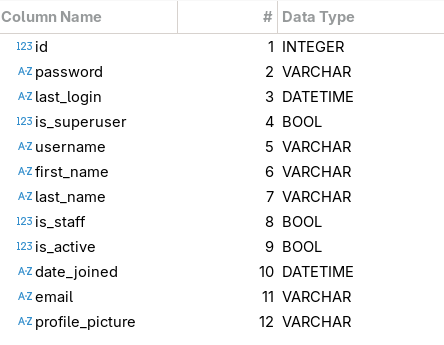
\includegraphics[width=0.8\textwidth]{images/user.png}
    \caption{Struttura della tabella degli Utenti.}
\end{figure}

Per controllare che l'untente sia registrato o faccia parte del gruppo dei moderatori o amministratori sono stati utilizzati i mixin di Django:

\begin{lstlisting}[language=bash]
    LoginRequiredMixin

    UserPassesTestMixin
    def test_func(self):
        return self.request.user.is_staff or self.request.user.groups.filter(name='Moderators').exists()
\end{lstlisting}

\clearpage

\section{Film}

I film sono il fulcro principale della piattaforma Plotwist. Ogni film ha attributi come titolo, regista, attori, generi, anno di uscita, trama e poster.
Gli utenti possono cercare film tramite vari filtri come genere, anno di uscita e regista.

Ogni film ha una pagina di dettaglio dove sono visualizzate tutte le informazioni e le recensioni degli utenti.
se un utente ha visto un film, può aggiungerlo alla propria watchlist per tenerne traccia.

Esiste una pagine che mostra i film aggiunti alla piattaforma dal utente moderatore loggato.
Quando si clicca sopra un film, si viene reindirizzati alla pagina di dettaglio del film.
Se il fim è statio aggiunto dal moderatore loggato, viene mostrato anche un pulsante per modificare o eliminare il film.

L'amministratore ha accesso alla modifica e cancellazione di tutti i film aggiunti da tutti i moderatori.
Tutti gli utenti posso aggiungere i film alla propria watchlist dalla pagina di dettaglio del film.

\begin{figure}[ht]
    \centering
    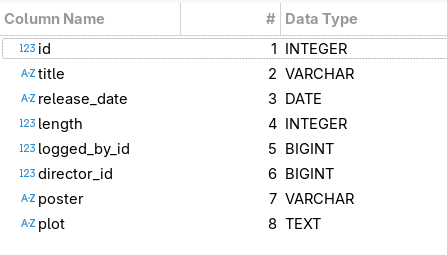
\includegraphics[width=0.8\textwidth]{images/movie.png}
    \caption{Struttura della tabella dei Film.}
\end{figure}

La watchlist è stata implementata con un campo ManyToMany nella tabella Movie che associa gli utenti ai film presenti nella loro watchlist.
L'aggiunta e rimozione di un film dalla watchlist avviene tramite una vista dedicata che verifica se il film è già presente nella watchlist dell'utente:
\begin{lstlisting}[language=bash]
def post(self, request, pk):
        movie = get_object_or_404(Movie, pk=pk)
        movie.watched_by.add(request.user)
        return redirect('movies:watchlist')
\end{lstlisting}

\clearpage



\section{Recensioni}

Nella pagina di dettaglio di ogni film, gli utenti registrati possono scrivere delle recensioni.
Ogni recensione è associata unicamente ad un utente e ad un film.

Gli utenti possono esprimere un voto da 1 a 10 e scrivere un commento testuale.
Viene visualizzato il voto medio del film calcolato in base a tutte le recensioni degli utenti.
Inoltre, gli utenti possono mettere o togliere "mi piace" alle recensioni degli altri utenti per indicare che trovano utile la recensione.
Ogni recensione mostra il numero totale di "mi piace" ricevuti,le recensioni con più "mi piace" vengono visualizzate in cima alla lista delle recensioni.

Una recensione può essere modificata o eliminata solo dall'utente che l'ha scritta o dall'amministratore della piattaforma.
Quando una recensione viene eliminata, tutti i "mi piace" associati a quella recensione vengono eliminati automaticamente, e il voto medio del film viene aggiornato di conseguenza.
Questo comporta un aggiornamento dei film nella classifica della home page se il voto medio cambia.

\begin{figure}[ht]
    \centering
    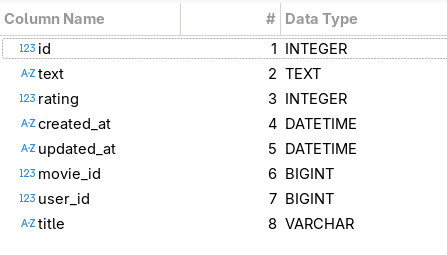
\includegraphics[width=0.8\textwidth]{images/review.png}
    \caption{Struttura della tabella delle Recensioni.}
\end{figure}

Per implementare la funzionalità di "mi piace" alle recensioni, è stata creata una tabella separata "Like" che associa gli utenti alle recensioni a cui hanno messo "mi piace".
Per stabilire se un utente ha messo "mi piace" ad una recensione, è stato creato un tag personalizzato nei template Django.

In \texttt{apps/reviews/templatetags/reviews\_extras.py}:

\begin{lstlisting}[language=bash]
@register.simple_tag
def has_liked(review, user):
    """Return True if the given user liked the review."""
    if not user or not user.is_authenticated:
        return False
    return review.likes.filter(user=user).exists()
\end{lstlisting}

\clearpage

In \texttt{apps/reviews/templatetags/reviews\_extras.py}:

\begin{lstlisting}[language=bash]
{% has_liked review user as user_liked %}
{% if user_liked %}
    <span> Hai messo like</span>
{% endif %}
\end{lstlisting}



\section{Raccomandazioni}

La piattaforma Plotwist utilizza un sistema di Content-Based Filtering che funziona nel seguente modo:

\begin{itemize}
    \item \textbf{Identificare i film preferiti dell'utente}: 
    il sistema estrae tutti i film che l'utente ha votato $\geq 7$ (su 10),
    se non ci sono film votati $\geq 7$, l'utente non riceve raccomandazioni.
    \item \textbf{Estrazione delle preferenze}: Dal set di film votati $\geq 7$, il sistema estrae tre tipi di caratteristiche:
    \begin{itemize}
        \item Generi preferiti: Tutti i generi dei film che l'utente ha votato
        \item Registi preferiti: Tutti i registi dei film che l'utente ha votato
        \item Attori preferiti: Tutti gli attori presenti nei film che l'utente ha votato
    \end{itemize}
    \item \textbf{Ricerca di film simili}: Il sistema cerca film che NON sono stati ancora recensiti dall'utente e che condividono:
    \begin{itemize}
        \item Almeno uno dei generi preferiti
        \item Almeno uno dei registi preferiti
        \item Almeno uno degli attori preferiti
    \end{itemize}
\end{itemize}

\begin{lstlisting}[language=bash]
user_reviewed_movies = Movie.objects.filter(
        reviews__user=user
        ).values_list('id', flat=True)

        recommendations = Movie.objects.filter(
            Q(genres__in=preferred_genres) |
            Q(director__in=preferred_directors) |
            Q(actors__in=preferred_actors)
        ).exclude(
            id__in=user_reviewed_movies
        ).annotate(
            avg_rating=Avg('reviews__rating')
        ).distinct().order_by('-avg_rating')
\end{lstlisting}

\chapter{Struttura del Database}
In questo capitolo viene mostrato lo schema ER semplificato del database di Plotwist.
Per gestire l'associazione molti-a-molti tra film e generi e tra filmm e attori, sono state create due tabelle intermedie "MovieGenre" e "MovieActor" che collegano i film ai rispettivi generi e attori.
Allo stesso modo, per gestire la watchlist degli utenti, è stata creata una tabella intermedia "Watchlist" che associa gli utenti ai film presenti nella loro watchlist.
\begin{figure}[ht]
    \centering
    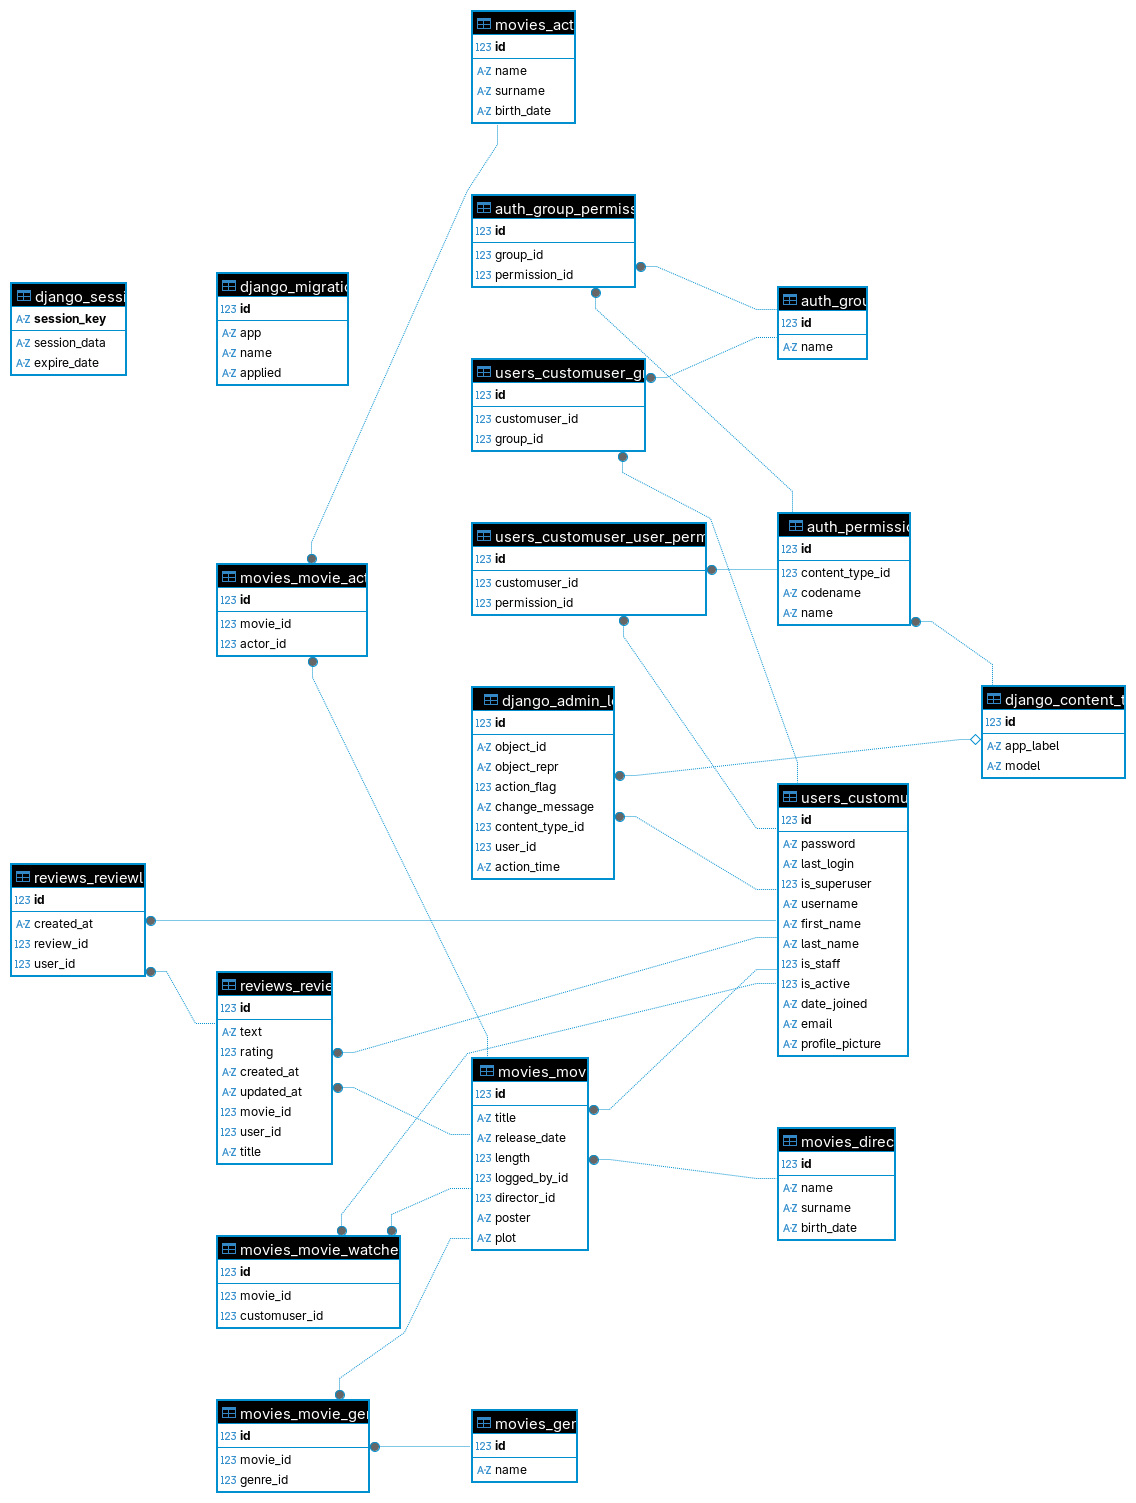
\includegraphics[width=0.8\textwidth]{images/uml.png}
    \caption{Schema ER del database.}
\end{figure}



\chapter{Test}

\begin{description}
    \item[test\_average\_rating\_no\_reviews] Verifica che il calcolo del voto medio di un film senza recensioni ritorni None.
    \item[test\_average\_rating\_single\_review] Verifica che il calcolo del voto medio di un film con una singola recensione ritorni il voto corretto.
    \item[test\_average\_rating\_multiple\_reviews] Verifica che il calcolo del voto medio di un film con più recensioni ritorni il valore corretto arrotondato a due decimali.
    \item[test\_average\_rating\_rounding] Verifica che il calcolo del voto medio di un film con recensioni che richiedono arrotondamento ritorni il valore corretto arrotondato a due decimali.
    \item[test\_average\_rating\_extreme\_values] Verifica che il calcolo del voto medio di un film con recensioni ai valori estremi (1 e 10) ritorni il valore corretto arrotondato a due decimali.
    \item[test\_movie\_detail\_view\_returns\_200] Verifica che la vista di dettaglio del film ritorni uno status code 200 (OK) per un film esistente.
    \item[test\_movie\_detail\_view\_uses\_correct\_template] Verifica che la vista di dettaglio del film utilizzi il template HTML corretto.
    \item[test\_movie\_detail\_contains\_movie\_data] Verifica che la vista di dettaglio del film contenga i dati corretti del film (titolo, regista, anno di uscita).
    \item[test\_movie\_detail\_contains\_reviews] Verifica che la vista di dettaglio del film contenga le recensioni associate al film.
    \item[test\_movie\_detail\_context\_data] Verifica che la vista di dettaglio del film fornisca i dati di contesto corretti (film, recensioni, voto medio).
    \item[test\_movie\_detail\_unauthenticated\_user] Verifica che un utente non autenticato possa accedere alla vista di dettaglio del film.
    \item[test\_movie\_detail\_authenticated\_not\_owner] Verifica che un utente autenticato che non è il proprietario del film possa accedere alla vista di dettaglio del film.
    \item[test\_movie\_detail\_authenticated\_owner] Verifica che un utente autenticato che è il proprietario del film possa accedere alla vista di dettaglio del film.
    \item[test\_movie\_detail\_average\_rating\_displayed] Verifica che il voto medio del film venga visualizzato correttamente nella vista di dettaglio del film.
    \item[test\_movie\_detail\_watchlist\_button\_authenticated] Verifica che il pulsante per aggiungere/rimuovere il film dalla watchlist venga visualizzato per un utente autenticato.
    \item[test\_movie\_detail\_404\_nonexistent\_movie] Verifica che la vista di dettaglio del film ritorni uno status code 404 (Not Found) per un film inesistente.
\end{description}



\begin{figure}[p]
    \centering
    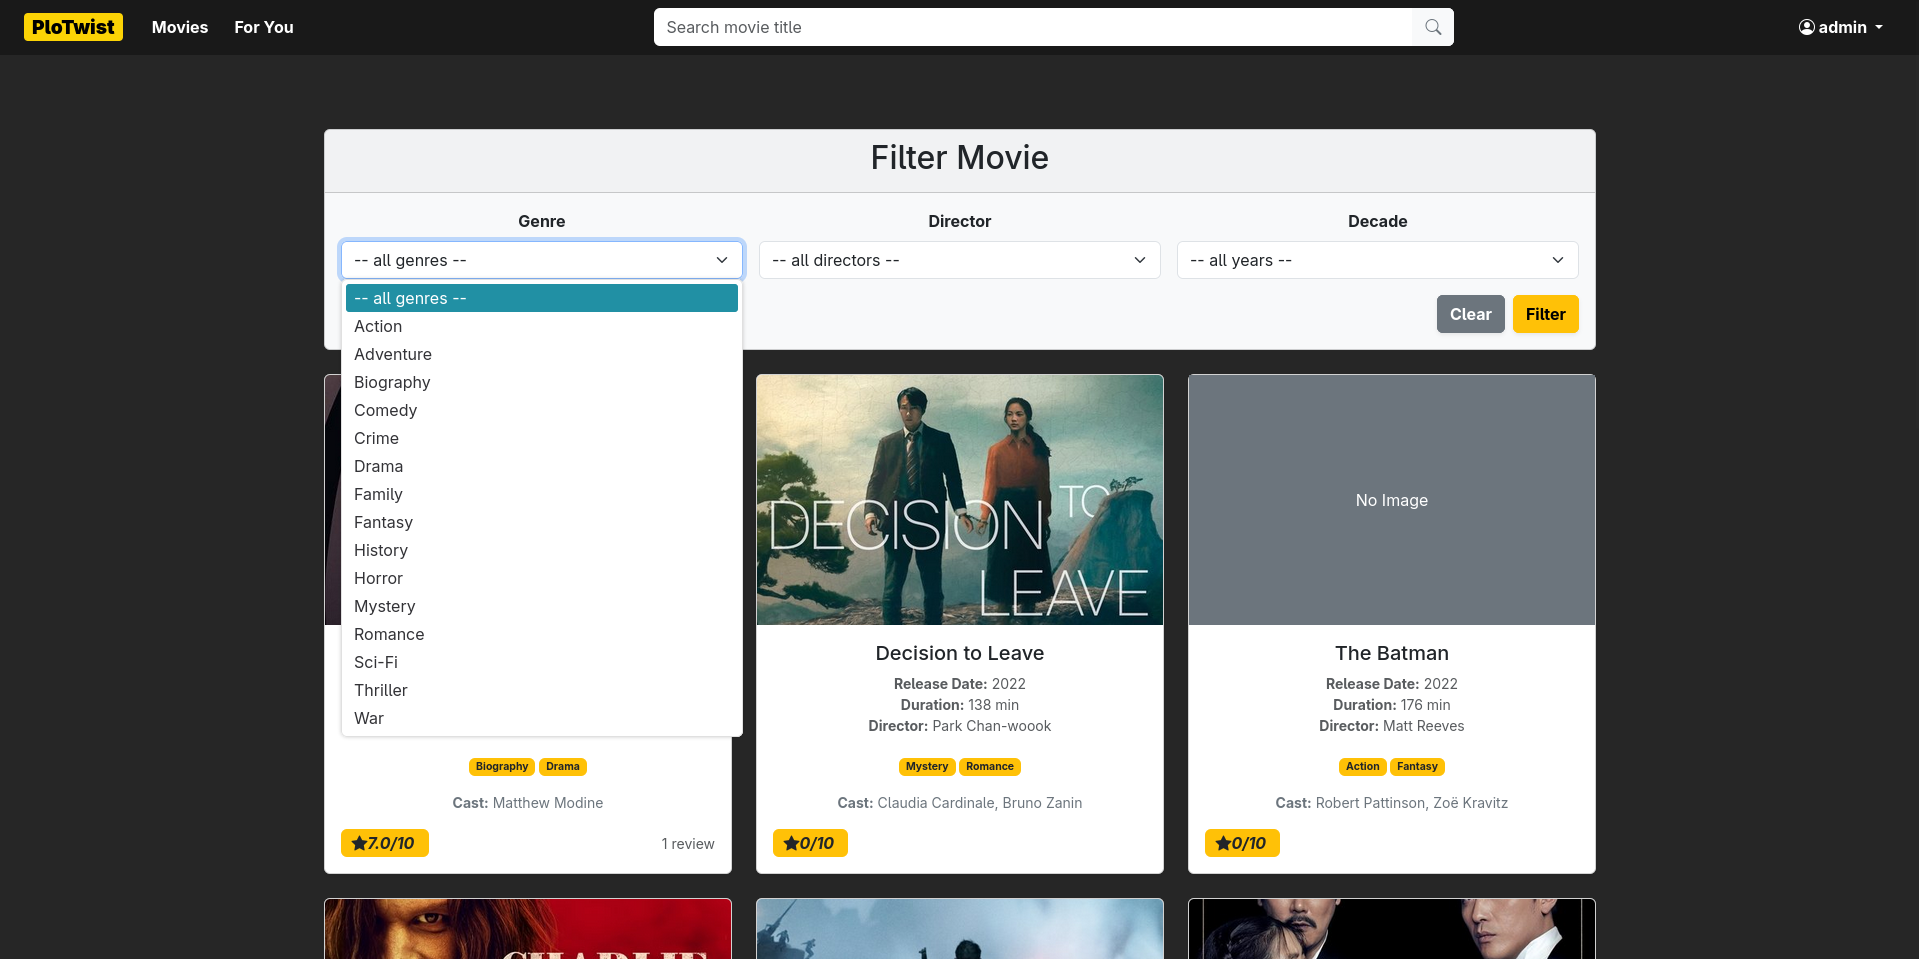
\includegraphics[width=1\textwidth]{images/filtro.png}
    \caption{Filtro per la ricerca dei film.}
\end{figure}

\clearpage

\begin{figure}[p]
    \centering
    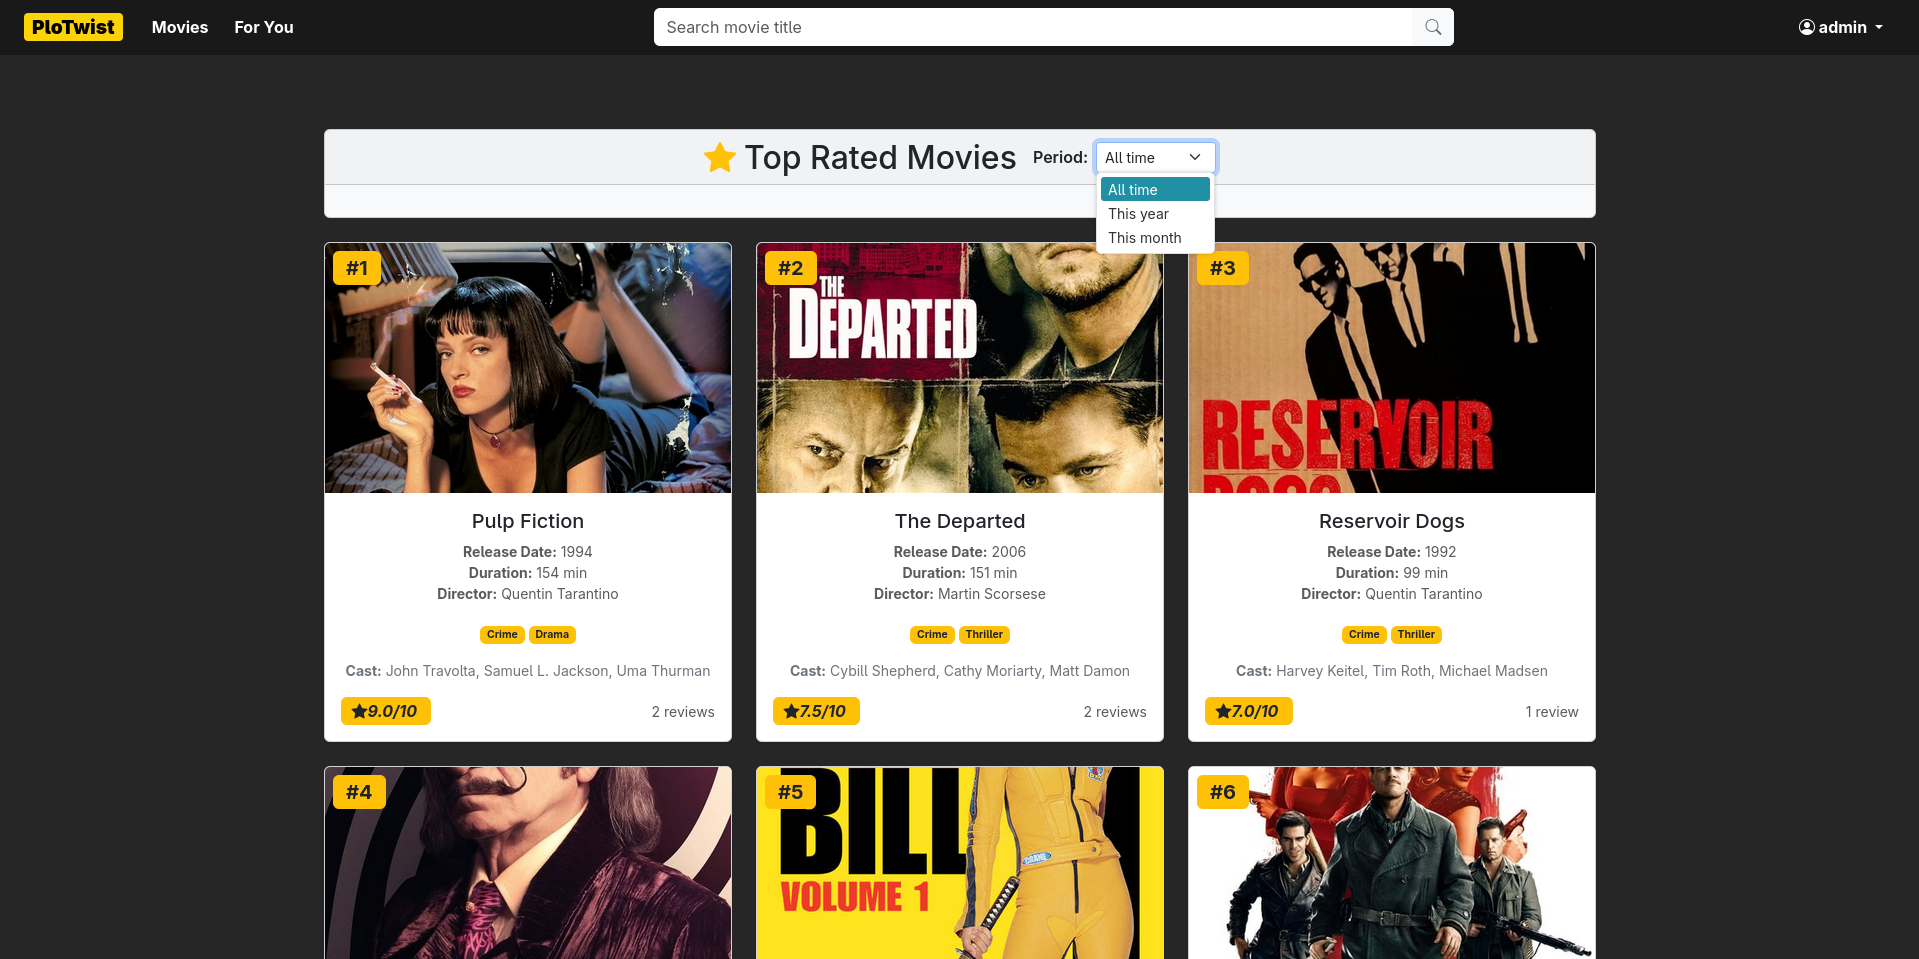
\includegraphics[width=1\textwidth]{images/filtro_iniziale.png}
    \caption{Filtro per la classifica dei film.}
\end{figure}

\end{document}